\documentclass[11pt]{article}

\usepackage[margin=1in]{geometry}
\usepackage{amsmath,amssymb,bm}
\usepackage{booktabs}
\usepackage{graphicx}
\usepackage{hyperref}
\usepackage{enumitem}
\usepackage{array}
\usepackage{caption}
\usepackage{float}

\graphicspath{{../figures/}}
\hypersetup{colorlinks=true, linkcolor=blue, citecolor=blue, urlcolor=blue}

\title{Fock-Resolved Qubit-State Inference for a Black-Box SQR Gate:\\
What Wait-and-Displacement Tomography Can and Cannot Recover}
\author{Autonomous cQED Research Platform}
\date{March 31, 2026}

\begin{document}
\maketitle

\begin{abstract}
We study whether a black-box selective qubit rotation can be validated without
reconstructing the full joint qubit-cavity process. The assumed calibrated
analysis operations are deliberately limited to a cavity displacement, free
dispersive waiting under known $(\chi,\chi')$, and ordinary qubit tomography.
The central target is the effective Fock-resolved qubit output state
$\rho_q^{(n,\mathrm{out})} \propto \langle n|\rho_{\mathrm{out}}|n\rangle$ on the
low-lying cavity manifolds. We combine an analytic identifiability analysis,
single-qubit maximum-likelihood tomography validation, synthetic inverse-problem
benchmarks, and pulse-level black-box case studies generated with
\texttt{cqed\_sim}. The positive result is that the weighted transverse sector
content $u_n = p_n (X_n + i Y_n)$ is recoverable: wait-only tomography is already
full-rank on that subspace, while the combined displacement-plus-wait protocol
is modestly more noise-robust in the tested grids. The negative result is that
the allowed measurements do not separate the Fock populations $p_n$ from the
sectorwise longitudinal components $Z_n$; displacement-only measurements reduce
to the ordinary qubit marginal, and an explicit gauge family shows that distinct
sets of $\{p_n,\rho_q^{(n)}\}$ generate identical recoverable data. The combined
protocol is nevertheless valuable because it turns cavity coherences into a
diagnostic residual: in an exact coherent benchmark the wait-only diagonal-model
residual remains at $1.6\times 10^{-16}$, whereas the combined residual rises to
$1.39\times 10^{-1}$. Pulse-level black-box tests show the same pattern. For
near-diagonal pulse-level outputs the combined protocol recovers the weighted
transverse sectors with errors below $3\times 10^{-3}$, but for coherent or
leaky outputs its large residual warns that the fitted Fock-resolved picture is
only an effective diagnostic. The experimentally defensible recommendation is
therefore to use the combined protocol when one wants both recovery of weighted
transverse sector data and a coherence/mismatch witness, while avoiding any
claim of direct $p_n$ or $Z_n$ recovery unless an additional cavity-sensitive
measurement primitive is added.
\end{abstract}

\section{Introduction}
Dispersive circuit quantum electrodynamics provides a natural route to
photon-number-conditioned qubit control, oscillator encodings, and selective
diagnostics of joint qubit-cavity dynamics \cite{blais2004cqed,heeres2015snap}.
In practice, however, a laboratory black-box gate may be available only through
its calibrated input-output behavior rather than through a trusted microscopic
pulse model. The question addressed here is not how to reconstruct the full
joint process, but instead how much of the low-lying Fock-resolved qubit action
can be inferred from a restricted set of post-gate analysis operations.

The allowed operations are intentionally weak: a calibrated displacement
$D(\alpha)$ on the cavity, free waiting under known dispersive parameters
$(\chi,\chi')$, and calibrated qubit tomography rotations followed by the usual
qubit readout. These ingredients are realistic in many cQED settings and fit
comfortably within standard qubit-state tomography practice
\cite{james2001measurement,lvovsky2009tomography}. They are also weaker than a
fully selective Fock-tagging primitive. That weakness is scientifically useful
because it forces the inverse problem to reveal exactly what information is and
is not available from such black-box validation.

The study therefore asks a sharply constrained question:
\begin{quote}
Given a black-box SQR, known dispersive waiting, calibrated displacement, and
ordinary qubit tomography, can one reliably infer the effective qubit output
state associated with each low-lying cavity Fock sector?
\end{quote}
The answer is mixed. A recoverable subspace exists and is experimentally useful,
but it is smaller than the optimistic target of full sector-resolved qubit-state
tomography.

\section{Problem Statement and Inference Targets}
We consider a post-gate joint state on a qubit plus cavity. Under the favorable
Fock-diagonal model,
\begin{equation}
\rho_{\mathrm{out}} =
\sum_{n=0}^{N-1} p_n |n\rangle\!\langle n| \otimes \rho_q^{(n)},
\label{eq:fockdiag}
\end{equation}
the sector state is parameterized as
\begin{equation}
\rho_q^{(n)} = \frac{1}{2}\left(I + X_n \sigma_x + Y_n \sigma_y + Z_n \sigma_z\right).
\label{eq:blochsector}
\end{equation}
The more general block model,
\begin{equation}
\rho_{\mathrm{out}} = \sum_{m,n=0}^{N-1} |m\rangle\!\langle n| \otimes A_{mn},
\label{eq:blockmodel}
\end{equation}
allows cavity coherences through the off-diagonal blocks $A_{mn}$ with
$m\neq n$.

The scientific target is not the full joint state in Eq.~\eqref{eq:blockmodel}.
Instead, we ask whether the measurements can recover the effective sector
marginals in Eq.~\eqref{eq:fockdiag}. It is therefore essential to distinguish
three different inference goals:
\begin{enumerate}[label=\arabic*.]
\item recovery of the weighted transverse sector content
$p_n X_n$ and $p_n Y_n$;
\item recovery of the normalized sector states $\rho_q^{(n)}$ themselves;
\item recovery of the full joint-state information, including cavity
coherences.
\end{enumerate}
Only the first goal is generally achievable under the stated constraints.

\section{Forward Model and Identifiability}
The calibrated analysis sequence is
\begin{equation}
\rho \mapsto U_{\mathrm{wait}}(t)\,
\left(I\otimes D(\alpha)\right)\rho
\left(I\otimes D^\dagger(\alpha)\right)\,
U_{\mathrm{wait}}^\dagger(t),
\end{equation}
with
\begin{equation}
U_{\mathrm{wait}}(t)=\sum_{m=0}^{N-1}
|m\rangle\!\langle m|\otimes R_z[\phi_m(t)],
\qquad
\phi_m(t)=\left[\chi m + \chi' m(m-1)\right]t.
\label{eq:waitunitary}
\end{equation}
For the Fock-diagonal model of Eq.~\eqref{eq:fockdiag}, the measured reduced
qubit state is
\begin{equation}
\rho_q^{\mathrm{meas}}(\alpha,t) =
\sum_{n=0}^{N-1} p_n \sum_{m=0}^{N-1}
P_{mn}(\alpha)\,
R_z[\phi_m(t)]\,\rho_q^{(n)}\,R_z^\dagger[\phi_m(t)],
\label{eq:diagforward}
\end{equation}
where
\begin{equation}
P_{mn}(\alpha)=|\langle m|D(\alpha)|n\rangle|^2.
\end{equation}
Equation~\eqref{eq:diagforward} implies
\begin{equation}
X(\alpha,t)+iY(\alpha,t)=
\sum_{n=0}^{N-1} u_n K_n(\alpha,t),
\qquad
u_n \equiv p_n(X_n+iY_n),
\label{eq:recoverablekernel}
\end{equation}
with
\begin{equation}
K_n(\alpha,t)=\sum_{m=0}^{N-1} P_{mn}(\alpha)e^{-i\phi_m(t)},
\end{equation}
while the longitudinal observable remains
\begin{equation}
Z(\alpha,t)=\sum_{n=0}^{N-1} p_n Z_n.
\label{eq:zcollapse}
\end{equation}

Two consequences are immediate.
\begin{enumerate}[label=\alph*)]
\item \textbf{Displacement-only data are uninformative for sector separation.}
When $t=0$, Eq.~\eqref{eq:diagforward} reduces to the ordinary reduced qubit
state because the local cavity unitary disappears under the partial trace.
\item \textbf{The protocol does not separate $p_n$ and $Z_n$.}
Equation~\eqref{eq:zcollapse} collapses all sectorwise longitudinal information
into a single scalar.
\end{enumerate}

For the general block model of Eq.~\eqref{eq:blockmodel}, the displacement
matrix elements mix off-diagonal cavity blocks into the reduced qubit signal:
\begin{equation}
\rho_q^{\mathrm{meas}}(\alpha,t)=
\sum_{m,n,r}
\langle r|D(\alpha)|m\rangle
\langle n|D^\dagger(\alpha)|r\rangle
R_z[\phi_r(t)]A_{mn}R_z^\dagger[\phi_r(t)].
\label{eq:blockforward}
\end{equation}
Hence cavity coherences are invisible to wait-only data ($\alpha=0$) but can
re-enter once displacement is applied.

\section{Numerical Methods}
\subsection{Single-qubit tomography engine}
The reusable single-qubit tomography block begins from the target rotation
\begin{equation}
U = R_x(\pi/3)R_z(\pi/4),
\end{equation}
acting on $|g\rangle\langle g|$. Three pre-measurement branches are used:
\begin{equation}
U_z = I,\qquad
U_x = R_y(-\pi/2),\qquad
U_y = R_x(\pi/2).
\end{equation}
The reconstructed state is parameterized with a Cholesky factor,
\begin{equation}
T =
\begin{pmatrix}
e^{s_1} & 0 \\
t_2 + i t_3 & e^{s_4}
\end{pmatrix},
\qquad
\rho(T)=\frac{T^\dagger T}{\mathrm{Tr}(T^\dagger T)},
\end{equation}
which enforces positivity by construction. We compare least-squares fitting of
the measured Pauli expectations to a binomial shot-noise maximum-likelihood
objective.

\subsection{Protocol grids and inverse solvers}
The main inverse study uses four active Fock sectors. The wait-only protocol
uses 11 wait times between $0$ and $0.35~\mu\mathrm{s}$; the combined protocol
uses a $5\times 9$ grid of displacements and waits; the displacement-only
protocol uses seven displacements at $t=0$. For the diagonal model, the
recoverable unknown vector is the $9$-parameter real vector containing the real
and imaginary parts of $u_n$ together with the single scalar
$\sum_n p_n Z_n$. Because Eq.~\eqref{eq:recoverablekernel} is linear in those
unknowns, the recoverable fit can be solved by both constrained least squares
and binomial maximum likelihood.

\subsection{Black-box case library}
The study uses three classes of validation cases.
\begin{enumerate}[label=\arabic*.]
\item \textbf{Controlled analytic cases:} ideal block-diagonal SQR outputs,
CPSQR-like conditional phases, and coherent companions with the same diagonal
sector marginals.
\item \textbf{Pulse-level near-diagonal cases:} an optimized multitone
black-box waveform synthesized on a six-level cavity truncation with a
two-level transmon.
\item \textbf{Failure-mode cases:} a short unoptimized waveform and a replay of
the optimized waveform on a three-level transmon model to expose leakage.
\end{enumerate}

\section{Results}
\subsection{Single-qubit baseline}
Figure~\ref{fig:baseline} shows the fidelity-versus-shot-count scaling of the
single-qubit tomography engine. The full-profile study reached a mean
maximum-likelihood fidelity of $0.9986$ at $10^4$ shots per branch, validating
the numerical tomography block before it was embedded in the joint inverse
problem.

\begin{figure}[H]
\centering
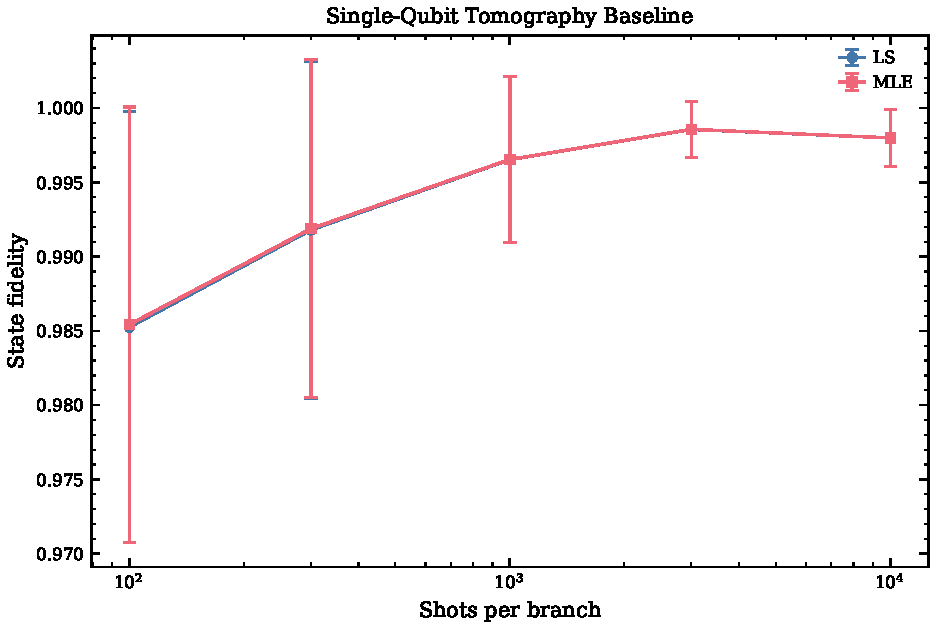
\includegraphics[width=0.72\linewidth]{single_qubit_fidelity_scaling}
\caption{Single-qubit baseline. The Cholesky-parameterized maximum-likelihood
reconstruction converges toward unit fidelity with the expected shot-noise
scaling and serves as the reusable building block for the Fock-resolved
inference layer.}
\label{fig:baseline}
\end{figure}

\subsection{Protocol identifiability and protocol comparison}
The identifiability audit is decisive. Wait-only and combined protocols both
have full transverse rank $8$ on the recoverable subspace, whereas the
displacement-only transverse rank collapses to $2$, corresponding to the
ordinary reduced-qubit aggregate. In the tested grids the wait-only design is
slightly better conditioned (condition number $1.21$ versus $2.34$), but the
combined protocol performs slightly better in noisy finite-shot inversion
because it averages over more informative settings.

At $10^4$ shots per setting, the mean weighted-transverse root-mean-square error
is $4.14\times 10^{-3}$ for wait-only, $2.95\times 10^{-3}$ for the combined
protocol, and $2.17\times 10^{-1}$ for displacement-only. Figure~\ref{fig:proto}
summarizes this comparison across the shot sweep.

\begin{figure}[H]
\centering
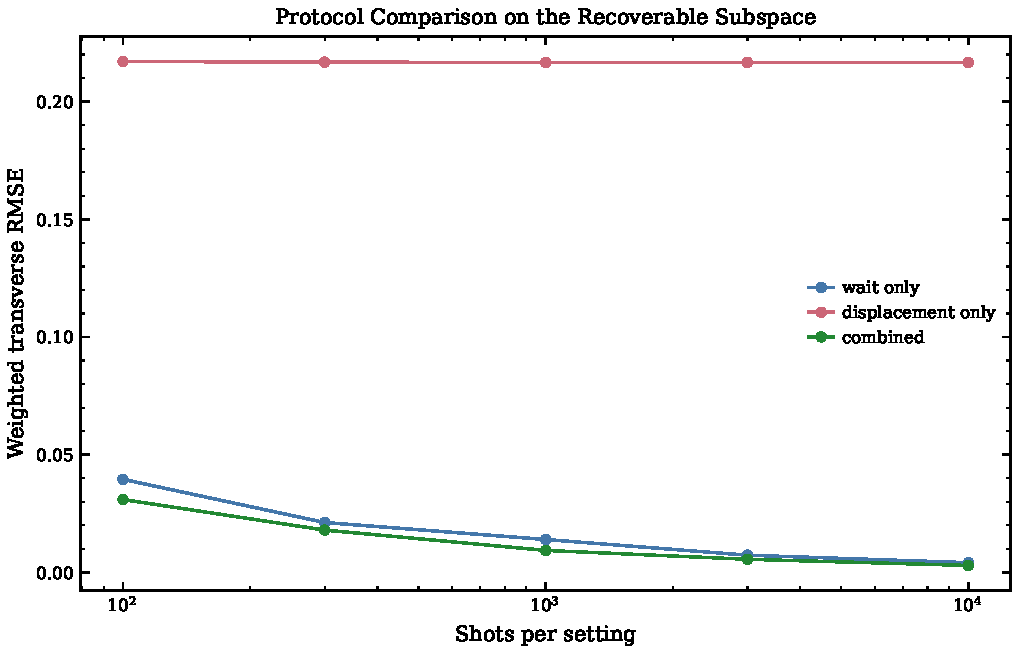
\includegraphics[width=0.74\linewidth]{protocol_comparison}
\caption{Protocol comparison on the recoverable weighted-transverse subspace.
Displacement-only measurements remain non-identifiable at every shot count.
Wait-only is already sufficient for recovery, while the combined protocol is
modestly more accurate in the tested finite-shot benchmarks.}
\label{fig:proto}
\end{figure}

\subsection{Coherence witness and explicit non-identifiability}
The strongest positive role of displacement is not the recovery of $p_n$ or
$Z_n$, but the exposure of cavity coherences. In an exact coherent benchmark
with the same diagonal sector marginals as the diagonal control case, the
wait-only residual remains at $1.6\times 10^{-16}$ because the off-diagonal
cavity blocks are invisible. The combined residual rises to $1.39\times 10^{-1}$,
whereas the diagonal control case remains at $2.8\times 10^{-16}$. The combined
protocol therefore functions as a sharp model-mismatch witness.

The negative result is equally strong. For the diagonal benchmark with
$z_{\mathrm{tot}}=0.1162$, we construct two distinct exact gauge-family
solutions that reproduce the same recoverable data:
\[
\bm{p}^{(1)}=(0.4448,\,0.2924,\,0.1260,\,0.1368),\qquad
\bm{p}^{(2)}=(0.3775,\,0.3373,\,0.1036,\,0.1816),
\]
even though the original populations are $(0.41,\,0.27,\,0.19,\,0.13)$.
Because these distinct sector decompositions yield identical $u_n$ and the same
$z_{\mathrm{tot}}$, the protocol cannot claim direct recovery of $\{p_n,Z_n\}$.

\begin{figure}[H]
\centering
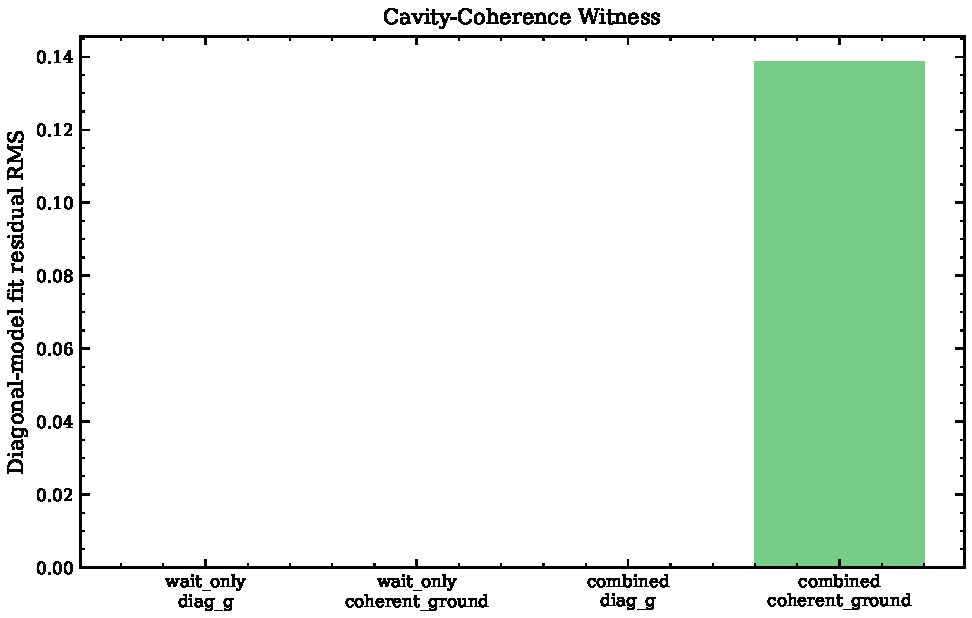
\includegraphics[width=0.70\linewidth]{coherence_witness_residuals}
\caption{Coherence-witness residuals. Wait-only fits remain exact for both the
diagonal and coherent benchmarks because cavity coherences do not enter the
reduced qubit data when $\alpha=0$. The combined protocol remains exact on the
diagonal case but produces a large residual on the coherent case, revealing the
hidden off-diagonal cavity structure.}
\label{fig:coherence}
\end{figure}

\subsection{Pulse-level black-box validation}
The pulse-level cases reproduce the same qualitative boundary. For the optimized
near-diagonal black-box cases, the combined protocol achieves weighted-sector
errors below $3\times 10^{-3}$ and outperforms wait-only. For example, on the
optimized cavity-mixture case with qubit $|g\rangle$, the combined weighted
root-mean-square error is $2.60\times 10^{-3}$, compared with
$9.63\times 10^{-3}$ for wait-only. On the optimized cavity-mixture case with
qubit $|+\rangle$, the corresponding errors are $3.38\times 10^{-3}$ and
$6.70\times 10^{-3}$.

The coherent and leaky cases behave differently for principled reasons. For the
optimized cavity-superposition case, wait-only still returns a small weighted
error of $8.76\times 10^{-3}$ because it is blind to cavity coherence, whereas
the combined fit error rises to $1.21\times 10^{-1}$ because the diagonal model
is no longer valid. For the replay on a three-level transmon, both protocols
fail on the recoverable weighted-sector metric, with errors between
$2.31\times 10^{-1}$ and $2.57\times 10^{-1}$, indicating that leakage moves the
output outside the effective qubit-sector model.

\begin{figure}[H]
\centering
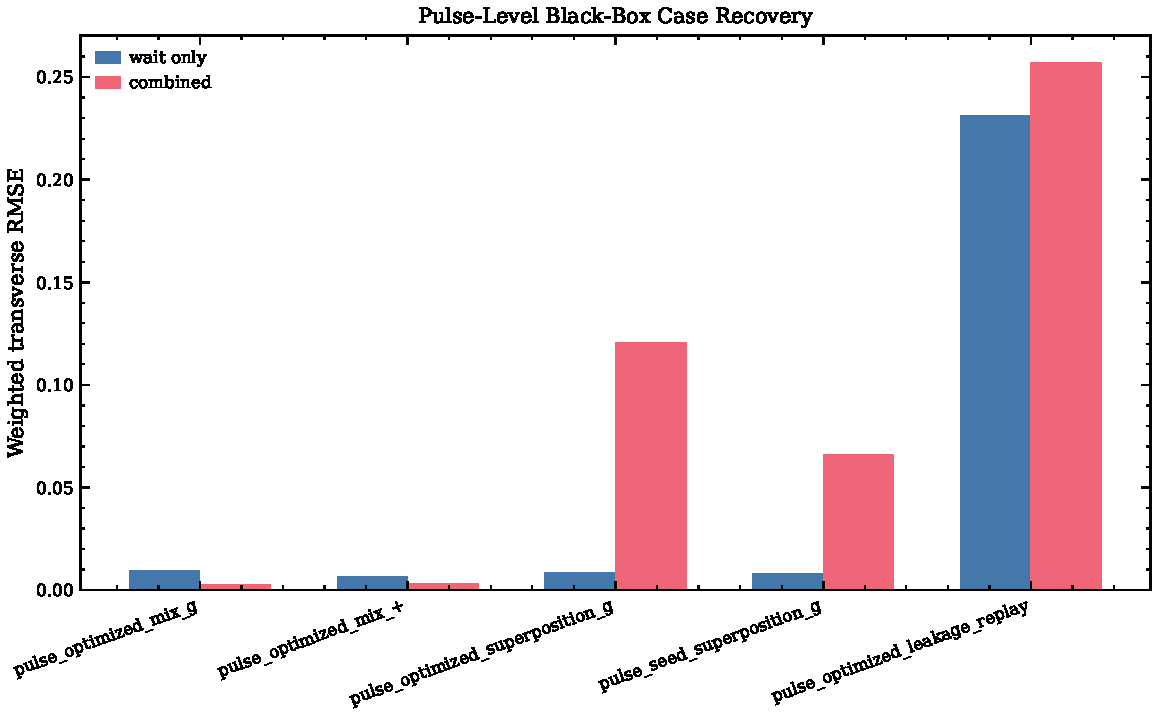
\includegraphics[width=0.78\linewidth]{pulse_case_recovery}
\caption{Pulse-level case recovery. Combined inference performs best on the
near-diagonal pulse-level black-box outputs, but it deliberately fails on the
coherent and leakage-sensitive cases because those outputs violate the diagonal
model assumed by the inverse solver.}
\label{fig:pulse}
\end{figure}

\subsection{Noise robustness and experimental recommendation}
Figure~\ref{fig:robust} summarizes the robustness sweep. Across shot noise,
rotation error, displacement calibration error, dispersive mismatch, and wait
decoherence, the combined protocol consistently matches or slightly improves on
wait-only for the diagonal benchmark. At $1500$ shots per setting, the mean
weighted-transverse error is $7.52\times 10^{-3}$ for the combined protocol and
$9.93\times 10^{-3}$ for wait-only under shot noise alone; under displacement
miscalibration the corresponding errors are $8.13\times 10^{-3}$ and
$1.17\times 10^{-2}$.

The practical recommendation is therefore two-tiered:
\begin{enumerate}[label=\arabic*.]
\item Use the combined displacement-plus-wait protocol as the primary
experimental workflow when one wants both high-fidelity weighted-transverse
sector recovery and an internal witness for cavity coherence or model mismatch.
\item If the combined residual is large, do not interpret the fitted
Fock-resolved states literally. In that regime the combined protocol has done
its most valuable job by demonstrating that the diagonal effective model has
failed. A wait-only fit may still serve as a lower-information diagnostic of the
weighted transverse sectors, but not as a full validation of the black-box
action.
\end{enumerate}

\begin{figure}[H]
\centering
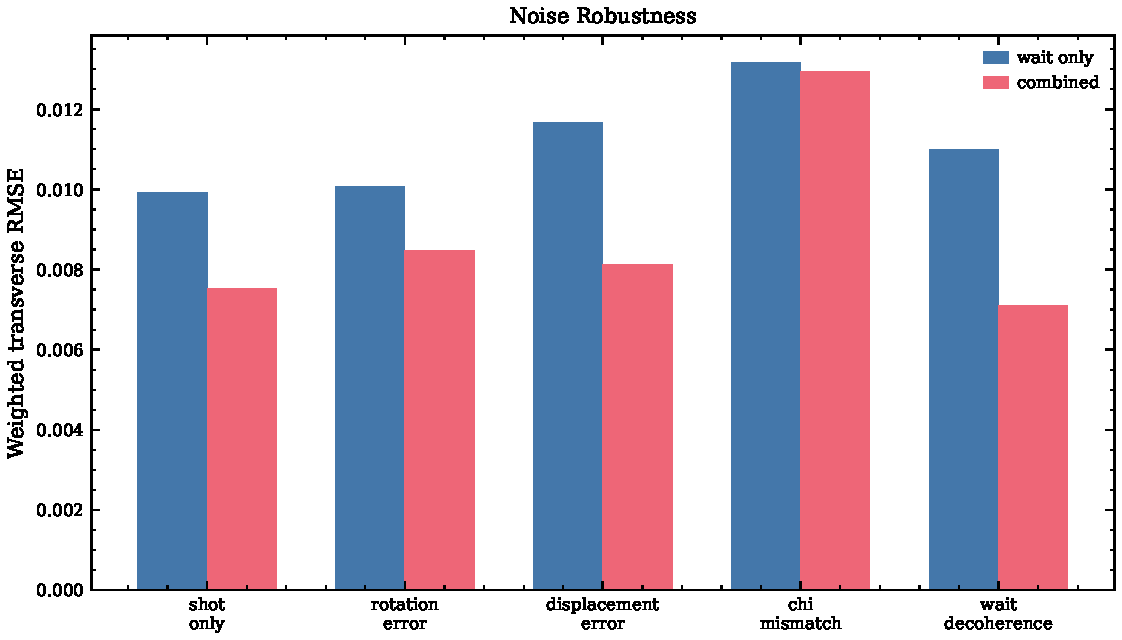
\includegraphics[width=0.78\linewidth]{robustness_sensitivity}
\caption{Noise robustness for the canonical diagonal benchmark. The combined
protocol is consistently as good as or better than wait-only on the recoverable
weighted-transverse metric, but its main additional value is the residual-based
coherence witness rather than the recovery of new identifiable parameters.}
\label{fig:robust}
\end{figure}

\section{Validation}
Three validation gates were enforced.
\paragraph{Sanity checks.}
The exact wait-only diagonal benchmark fits to machine precision.
Displacement-only remains rank-deficient. The coherent benchmark is invisible to
wait-only but exposed by the combined protocol.

\paragraph{Convergence.}
The exact recoverable fit remains at or below $10^{-7}$ weighted-transverse
error under denser combined grids and modest changes in the kernel truncation.

\paragraph{Pulse-level consistency.}
The near-diagonal pulse-level cases follow the same identifiability logic as
the analytic benchmarks, while the leakage replay fails in the expected
direction.
Because this is an original identifiability and protocol-design study rather
than a reproduction of a prior benchmark, a literature-error comparison is not
the relevant validation metric here.

\section{Limitations and Future Work}
The central limitation is structural rather than numerical: the measurement set
does not identify $p_n$ or sector-resolved $Z_n$. No amount of additional
least-squares or maximum-likelihood tuning will change that. A future protocol
that adds a cavity-sensitive primitive such as parity, selective tagging, or a
direct cavity readout could remove that nullspace.

The pulse-level library is also intentionally representative rather than
exhaustive. It contains a near-diagonal optimized waveform, a short unoptimized
waveform, and a leakage replay. A larger survey over durations, detunings, and
decoherence models would sharpen the engineering recommendation but would not
change the identifiability boundary established by the analytic forward model.

\section{Conclusion}
Black-box SQR validation with calibrated displacement, dispersive waiting, and
ordinary qubit tomography is scientifically useful, but only if one states the
inverse target correctly. The protocol does \emph{not} recover the full
Fock-resolved qubit state in the sense of separate populations $p_n$ and
sectorwise longitudinal components $Z_n$. It \emph{does} recover the weighted
transverse sector amplitudes $u_n = p_n(X_n+iY_n)$, and it does so accurately in
both analytic and pulse-level near-diagonal cases. Moreover, the combined
protocol supplies a valuable residual-based witness for hidden cavity coherence
or leakage. The experimentally honest conclusion is therefore that the protocol
is trustworthy as a weighted-transverse black-box diagnostic and as a coherence
witness, but not as a complete sector-resolved tomography protocol without an
additional cavity-sensitive measurement primitive.

\appendix

\section{Detailed Results and Data}
\subsection{Protocol summary}
\begin{table}[H]
\centering
\caption{Mean weighted-transverse root-mean-square error for the canonical
diagonal benchmark under maximum-likelihood fitting.}
\begin{tabular}{>{\raggedright}p{0.27\linewidth}ccc}
\toprule
Shots per setting & Wait-only & Displacement-only & Combined \\
\midrule
$10^2$   & $3.95\times 10^{-2}$ & $2.17\times 10^{-1}$ & $3.10\times 10^{-2}$ \\
$3\times 10^2$ & $2.12\times 10^{-2}$ & $2.17\times 10^{-1}$ & $1.80\times 10^{-2}$ \\
$10^3$   & $1.40\times 10^{-2}$ & $2.17\times 10^{-1}$ & $9.35\times 10^{-3}$ \\
$3\times 10^3$ & $7.33\times 10^{-3}$ & $2.17\times 10^{-1}$ & $5.58\times 10^{-3}$ \\
$10^4$   & $4.14\times 10^{-3}$ & $2.17\times 10^{-1}$ & $2.95\times 10^{-3}$ \\
\bottomrule
\end{tabular}
\end{table}

\subsection{Exact gauge-family examples}
\begin{table}[H]
\centering
\caption{Two exact gauge-family solutions with identical recoverable data for
the diagonal benchmark used in the non-identifiability audit.}
\begin{tabular}{cc}
\toprule
Solution 1 populations & Solution 2 populations \\
\midrule
$(0.4448,\ 0.2924,\ 0.1260,\ 0.1368)$ &
$(0.3775,\ 0.3373,\ 0.1036,\ 0.1816)$ \\
\bottomrule
\end{tabular}
\end{table}

\subsection{Representative pulse-level outcomes}
\begin{table}[H]
\centering
\caption{Pulse-level weighted-transverse errors for representative black-box
cases.}
\begin{tabular}{>{\raggedright}p{0.40\linewidth}cc}
\toprule
Case & Wait-only RMSE & Combined RMSE \\
\midrule
Optimized cavity mixture, qubit $|g\rangle$ & $9.63\times 10^{-3}$ & $2.60\times 10^{-3}$ \\
Optimized cavity mixture, qubit $|+\rangle$ & $6.70\times 10^{-3}$ & $3.38\times 10^{-3}$ \\
Optimized cavity superposition, qubit $|g\rangle$ & $8.76\times 10^{-3}$ & $1.21\times 10^{-1}$ \\
Short seed waveform, cavity superposition, qubit $|g\rangle$ & $7.95\times 10^{-3}$ & $6.60\times 10^{-2}$ \\
Optimized waveform replay on a three-level transmon & $2.31\times 10^{-1}$ & $2.57\times 10^{-1}$ \\
\bottomrule
\end{tabular}
\end{table}

\begin{figure}[H]
\centering
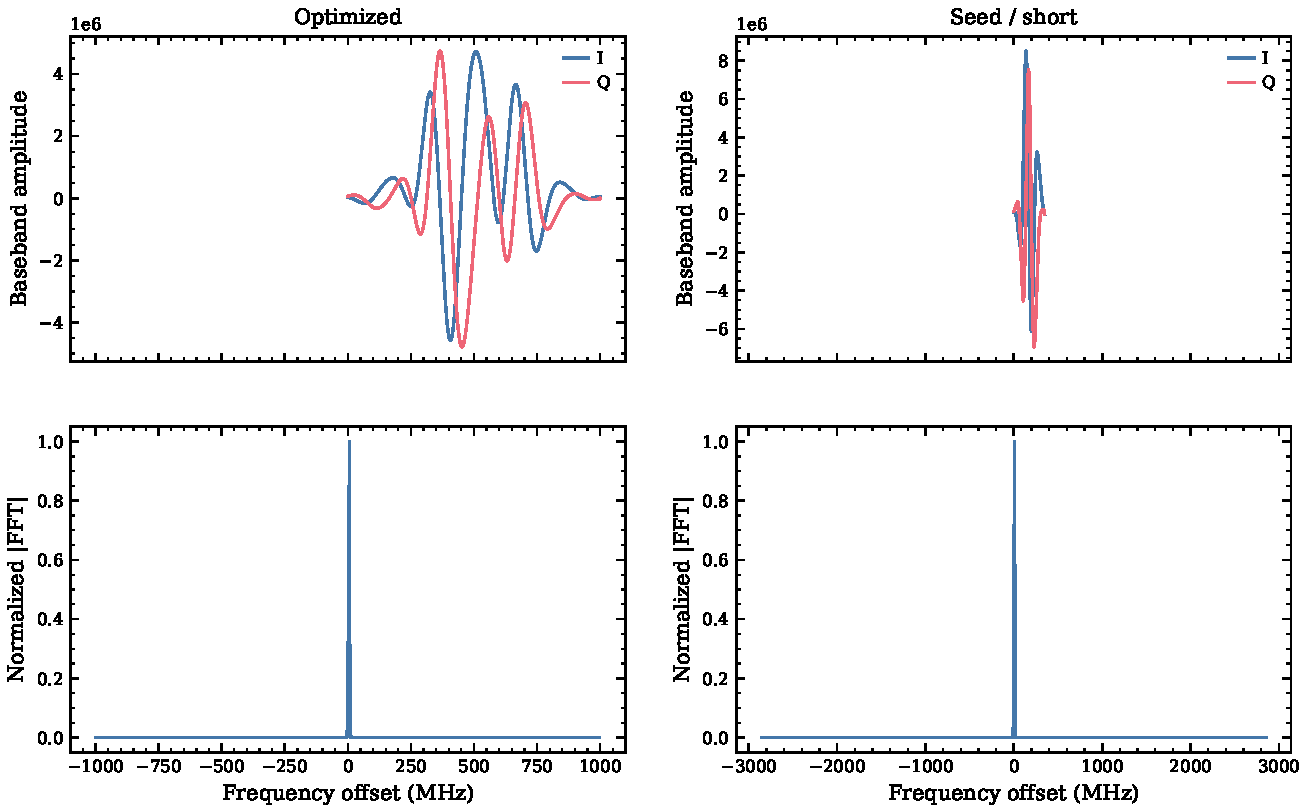
\includegraphics[width=0.82\linewidth]{waveform_examples}
\caption{Representative optimized and seed multitone waveforms together with
their spectra. These are the pulse-level black-box instances used in the
numerical validation study.}
\end{figure}

\begin{figure}[H]
\centering
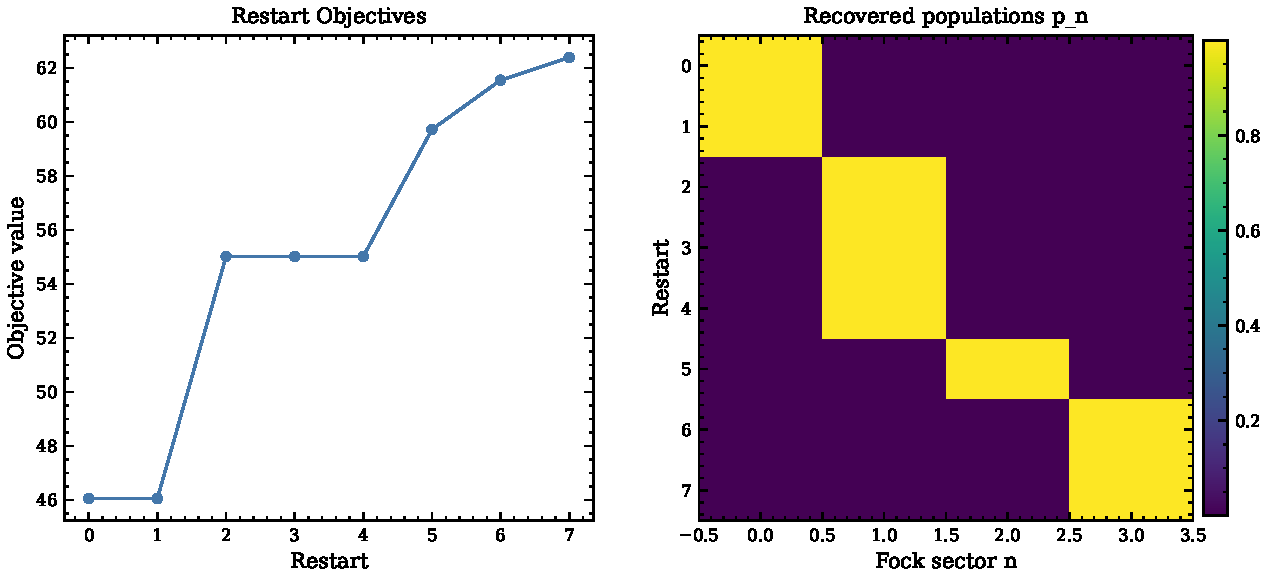
\includegraphics[width=0.75\linewidth]{full_state_nonuniqueness}
\caption{Restart-based full-state fit diagnostic. The broad spread of recovered
population assignments complements the explicit gauge-family construction and
illustrates the non-identifiability of the full $\{p_n,\rho_q^{(n)}\}$ model
under the restricted measurement set.}
\end{figure}

\section{Reproducibility}
The study is reproducible from the saved machine-readable outputs, figures, and
notebook in the study directory. The main execution entry point is
\texttt{scripts/run\_study.py}; the saved outputs are checked by
\texttt{scripts/validate\_results.py}; and the end-to-end interactive workflow is
documented in \texttt{scripts/reproducibility\_notebook.ipynb}. The notebook
exposes the main tunable parameters near the top and can rerun the study or
simply reload the saved results.

\bibliographystyle{unsrt}
\bibliography{references}

\end{document}
